% Sanctaphrax: Formal Verification of Luxembourg Fund Law
% A Catala Proof-of-Concept
%
% Author: Aymane Bengrina, Studio Alticcio
% Date: January 2025

\documentclass[10pt,twocolumn]{article}

% ============================================================================
% FONTS AND TYPOGRAPHY
% ============================================================================
\usepackage[utf8]{inputenc}
\usepackage[T1]{fontenc}
\usepackage{lmodern}              % Latin Modern fonts (clean, professional)
\usepackage[scaled=0.9]{helvet}   % Helvetica for sans-serif
\usepackage{microtype}            % Microtypographic improvements
\usepackage{lettrine}             % Drop caps for section openers

% ============================================================================
% CORE PACKAGES
% ============================================================================
\usepackage{amsmath,amssymb}
\usepackage{graphicx}
\usepackage[colorlinks=true,citecolor=darkblue,linkcolor=darkblue,urlcolor=darkblue]{hyperref}
\usepackage{xcolor}
\usepackage{listings}
\usepackage{booktabs}
\usepackage{longtable}
\usepackage{tikz}
\usetikzlibrary{decorations.pathreplacing,calc,positioning,shapes.geometric,arrows.meta,backgrounds,shadows}
\usepackage{geometry}
\usepackage[numbers,sort&compress]{natbib}
\usepackage{float}
\usepackage{caption}
\usepackage{subcaption}
\usepackage{enumitem}
\usepackage{fancyhdr}
\usepackage{setspace}

% ============================================================================
% PAGE GEOMETRY
% ============================================================================
\geometry{
  letterpaper,
  margin=0.85in,
  columnsep=0.3in,
  top=1in,
  bottom=1in
}

% ============================================================================
% COLORS
% ============================================================================
\definecolor{darkblue}{RGB}{0,51,102}
\definecolor{catalaKeyword}{RGB}{0,51,128}
\definecolor{catalaComment}{RGB}{96,96,96}
\definecolor{catalaString}{RGB}{128,0,0}
\definecolor{catalaScope}{RGB}{102,0,102}
\definecolor{codeBackground}{RGB}{248,248,248}
\definecolor{accentGreen}{RGB}{0,128,64}
\definecolor{accentOrange}{RGB}{204,102,0}

% ============================================================================
% LISTINGS CONFIGURATION (Catala)
% ============================================================================
\lstdefinelanguage{catala}{
  keywords={declaration, structure, enumeration, scope, input, output, internal,
            content, data, equals, under, condition, consequence, exception,
            definition, rule, with, pattern, match, if, then, else, and, or, not,
            let, in, true, false, Some, None, boolean, integer, decimal, money, text},
  keywordstyle=\color{catalaKeyword}\bfseries,
  sensitive=true,
  comment=[l]{\#},
  commentstyle=\color{catalaComment}\itshape,
  stringstyle=\color{catalaString},
  morestring=[b]",
  emphstyle=\color{catalaScope}\bfseries,
  emph={FundCharacteristics, AIFDefinition, ExclusionCheck, AIFExclusions,
        InvestorProfile, ProfessionalInvestorStatus, RAIFInvestorProfile,
        WellInformedInvestorStatus, RAIFStructure, RAIFCompliance,
        PermittedInvestmentDef, DefinitionConsistency, LargeUndertakingTest,
        PerSeProfessionalCategory, ExclusionCategory, LegalForm, AIFMType,
        InconsistencySeverity, FeeDefinition, FeeConsistency, AIFMDelegation,
        AIFMDelegationCompliance},
  basicstyle=\ttfamily\footnotesize,
  breaklines=true,
  breakatwhitespace=true,
  frame=single,
  framerule=0.5pt,
  rulecolor=\color{gray!40},
  backgroundcolor=\color{codeBackground},
  numbers=left,
  numberstyle=\tiny\color{gray},
  numbersep=8pt,
  tabsize=2,
  showstringspaces=false,
  xleftmargin=2em,
  framexleftmargin=1.5em,
  aboveskip=1em,
  belowskip=0.8em,
}
\lstset{language=catala}

% ============================================================================
% CAPTION STYLING
% ============================================================================
\captionsetup{
  font=small,
  labelfont=bf,
  labelsep=period,
  margin=1em
}

% ============================================================================
% HEADER/FOOTER
% ============================================================================
\pagestyle{fancy}
\fancyhf{}
\fancyhead[L]{\small\textit{Sanctaphrax: Formal Verification of Luxembourg Fund Law}}
\fancyhead[R]{\small\thepage}
\renewcommand{\headrulewidth}{0.4pt}
\fancypagestyle{plain}{
  \fancyhf{}
  \fancyfoot[C]{\small\thepage}
  \renewcommand{\headrulewidth}{0pt}
}

% ============================================================================
% CUSTOM COMMANDS
% ============================================================================
\newcommand{\catala}{\textsc{Catala}}
\newcommand{\aifmd}{\textsc{aifmd}}
\newcommand{\raif}{\textsc{raif}}
\newcommand{\mifid}{\textsc{MiFID~II}}
\newcommand{\bigO}[1]{\ensuremath{\mathcal{O}(#1)}}

% ============================================================================
% TITLE AND AUTHOR
% ============================================================================
\title{%
  \vspace{-1.5em}
  \textbf{\Large Sanctaphrax: Formal Verification of Luxembourg Fund Law}\\[0.3em]
  \large A \catala{} Proof-of-Concept
}

\author{%
  \textbf{Aymane Bengrina}\\
  Studio Alticcio\\
  \texttt{aymane@alticc.io}
}

\date{January 2025}

% ============================================================================
% DOCUMENT
% ============================================================================
\begin{document}

\twocolumn[
  \begin{@twocolumnfalse}
    \maketitle
    \vspace{-1em}

    \begin{abstract}
      \noindent\textbf{Background.} Legal compliance in modern investment fund structures is fundamentally a distributed consistency problem. A typical Luxembourg Reserved Alternative Investment Fund comprises dozens of interlocking documents---Limited Partnership Agreements, AIFM Agreements, side letters---each imposing constraints on the others.

      \smallskip
      \noindent\textbf{Problem.} Current manual verification scales linearly with document count (\bigO{N}), while inter-document cross-reference complexity scales quadratically (\bigO{N^2}). This creates ``legal bugs'': silent inconsistencies that remain dormant until a liquidity event or regulatory audit.

      \smallskip
      \noindent\textbf{Approach.} We present \textbf{Sanctaphrax}, a formal verification framework for Luxembourg fund law based on the \catala{} domain-specific language. We formalize key provisions of the Alternative Investment Fund Managers Directive (\aifmd{}) and the Reserved Alternative Investment Fund (\raif{}) Law, translating 150+ lines of regulation into executable, verifiable logic.

      \smallskip
      \noindent\textbf{Results.} We demonstrate that while arithmetic and logical provisions can be strictly verified, approximately 15\% of rules exhibit irreducible semantic ambiguity (``open texture'') that resists formalization. Our contributions include: (1)~a formal semantics for the \aifmd{} ``AIF'' definition, (2)~a Professional Investor eligibility oracle unifying \mifid{} and \raif{} Law, (3)~an automated cross-reference verification engine for document consistency, and (4)~a systematic categorization of legal ``bugs'' undetectable by traditional review.

      \smallskip
      \noindent\textbf{Keywords:} formal verification, computational law, \catala{}, \aifmd{}, fund structures, Luxembourg, default logic
    \end{abstract}
    \vspace{1.5em}
  \end{@twocolumnfalse}
]

%% Main content
% Section 1: Introduction

\section{Introduction}
\label{sec:introduction}

\lettrine[lines=2, lhang=0.15, loversize=0.1]{T}{he defining feature} of modern investment funds is not their asset strategy, but their documentary complexity. A standard Luxembourg Reserved Alternative Investment Fund (\raif{}) structure is not a single entity but a \textit{network} of interlocking legal agreements: a Limited Partnership Agreement (LPA), an AIFM Agreement, a Depositary Agreement, an Administration Agreement, and dozens of side letters granting individual investors bespoke terms. Each document imposes constraints on the others; a fee cap negotiated in a side letter must propagate to the Net Asset Value calculation logic in the Administration Agreement, which must align with the waterfall provisions in the LPA.

Currently, the consistency of this distributed system is verified manually. This approach is fundamentally non-scalable. As the number of documents ($N$) grows, the number of potential cross-references grows as \bigO{N^2}. For a typical structure with 50+ documents, manual verification relies on heuristics---trust, precedent, and sample-checking---rather than exhaustive proof. This creates what we term \textbf{``legal bugs''}: silent inconsistencies that remain dormant until a liquidity event, regulatory audit, or investor dispute triggers a crisis.

\subsection{The Case for Formal Verification}

We posit that fund law is amenable to \textbf{formal verification}. Unlike criminal law, which relies heavily on reasonable person standards, or constitutional law, which involves balancing abstract principles, fund law is largely \textit{structural} and \textit{arithmetic}. It deals with:

\begin{itemize}[nosep,leftmargin=1.5em]
  \item \textbf{Thresholds}: Assets under Management $\geq$ €100M triggers full \aifmd{} scope
  \item \textbf{Binary states}: Authorized vs.\ Registered AIFM status
  \item \textbf{Precise definitions}: Professional Investor per \mifid{} Annex~II
  \item \textbf{Algorithmic calculations}: Waterfall distributions, carried interest
\end{itemize}

These characteristics suggest that significant portions of fund law can be encoded as executable specifications that compile to provably correct implementations.

\subsection{Contributions}

In this work, we present \textbf{Sanctaphrax}, a proof-of-concept formalization of Luxembourg fund law using \textbf{\catala{}}~\cite{merigoux2021catala}. \catala{} is a domain-specific language (DSL) for literate programming that compiles law into correct-by-construction executable artifacts. It uses \textbf{default logic} to handle the general-case/exception structure typical of legislative texts---precisely the structure that dominates fund regulation.

Our contributions are as follows:

\begin{enumerate}[nosep,leftmargin=1.5em]
  \item We provide the first formal specification of the \textbf{Definition of an AIF} under \aifmd{} Article~4(1)(a), explicitly documenting the interpretive choices required.

  \item We implement a \textbf{Professional Investor eligibility oracle} that unifies \mifid{} and \raif{} Law requirements into a single decidable procedure.

  \item We demonstrate an automated \textbf{Cross-Reference Verification} mechanism that detects definition inconsistencies across separate fund documents.

  \item We analyze the \textbf{limits of formalization}, identifying and categorizing the approximately 15\% of provisions where human judgment cannot be replaced by code.
\end{enumerate}

\subsection{Approach and Limitations}

Unlike Large Language Model (LLM) approaches which \textit{predict} likely legal text based on statistical patterns, our approach provides \textbf{provable guarantees}. If the specification compiles and the inputs match the real-world situation, the conclusion follows \textit{deductively} from the encoded law. There is no hallucination, no probabilistic uncertainty in the reasoning chain.

However, we are explicit about what formal verification does \textit{not} provide:

\begin{itemize}[nosep,leftmargin=1.5em]
  \item It does not guarantee that our encoding matches the ``true'' legal meaning
  \item It does not replace the judgment required for open-textured concepts
  \item It does not predict how a court or regulator would interpret ambiguous provisions
\end{itemize}

The value lies in \textit{locating} where human judgment is required, not in replacing it. A specification that flags ``these two definitions of Permitted Investment differ'' allows a human to determine whether the difference is acceptable. The machine surfaces the question; the lawyer answers it.

\subsection{Paper Organization}

Section~\ref{sec:background} introduces \catala{} and default logic, explaining why fund law is a suitable domain. Sections~\ref{sec:aif}--\ref{sec:crossref} present our four specifications: AIF definition, Professional Investor eligibility, \raif{} structural requirements, and cross-reference verification. Section~\ref{sec:findings} analyzes where formalization breaks down. Section~\ref{sec:implications} discusses implications for practitioners, regulators, and researchers. Section~\ref{sec:questions} poses open questions. Section~\ref{sec:conclusion} concludes.

% Section 2: Background

\section{Background}
\label{sec:background}

\subsection{Catala: A Domain-Specific Language for Law}
\label{sec:catala}

\catala{} was developed by Merigoux et al.\ at INRIA to encode legal rules in executable form while preserving the structure of legal reasoning~\cite{merigoux2021catala}. Unlike general-purpose programming languages, \catala{} was designed with specific features that mirror legal text:

\paragraph{Literate Programming.} Legal text and code appear together in the same document. The statute or regulation is quoted verbatim, then encoded immediately below. This maintains \textit{traceability} between source and specification---every line of code can be traced to a specific legal provision.

\paragraph{Default Logic.} \catala{} implements a form of default logic~\cite{reiter1980logic} where general rules can be overridden by exceptions. This matches the structure of virtually all legislation: a general rule, followed by exceptions, possibly with exceptions to exceptions. The \texttt{exception} keyword makes this structure explicit:

\begin{lstlisting}
definition is_professional equals false

exception definition is_professional
  under condition investor.category = CreditInstitution
  consequence equals true
\end{lstlisting}

\paragraph{Formally Verified Compiler.} The \catala{} compiler has been partially verified using the F* proof assistant. The translation from \catala{} source to executable code is provably correct---if the specification is semantically well-formed, the execution will preserve that semantics.

\paragraph{Multiple Backends.} \catala{} compiles to Python, OCaml, and JavaScript, allowing integration with existing legal technology systems, web applications, and analytical tools.

\subsection{Default Logic and Legal Reasoning}
\label{sec:default-logic}

Lawsky argues persuasively that statutory reasoning is fundamentally \textit{defeasible}~\cite{lawsky2017logic}: conclusions hold unless some exception applies. Classical first-order logic struggles with this pattern. Consider the structure of tax law:

\begin{quote}
\textit{All income is taxable.}\\
\textbf{Except}: Certain deductions reduce taxable income.\\
\textbf{Unless}: The alternative minimum tax disallows those deductions.\\
\textbf{Except}: Specific exemptions may still apply under AMT.
\end{quote}

In classical logic, encoding this requires elaborate universal quantification with deeply nested negated conditions. In default logic, we express the \textit{structure} directly: a base rule, subject to exceptions, which are themselves subject to further exceptions. The semantics handles the interaction automatically.

\catala{} makes this explicit through exception chains. If multiple exceptions apply, the compiler detects the conflict and requires explicit prioritization---there are no silent ambiguities.

\subsection{Why Fund Law?}
\label{sec:why-fund-law}

Fund regulation exhibits precisely the default/exception hierarchy that \catala{} was designed to handle:

\begin{itemize}[nosep,leftmargin=1.5em]
  \item \textbf{\aifmd{}} provides general EU-wide rules for alternative investment funds
  \item \textbf{National Law} (\raif{} Law, AIFM Law) provides Luxembourg-specific exceptions and elaborations
  \item \textbf{CSSF Circulars} provide regulatory guidance interpreting the law (further exceptions and clarifications)
  \item \textbf{Fund Documents} (LPA, AIFM Agreement) provide fund-specific rules within regulatory limits
  \item \textbf{Side Letters} provide LP-specific exceptions to fund documents
\end{itemize}

This creates a five-layer exception hierarchy, visualized in Figure~\ref{fig:hierarchy} (Appendix~\ref{app:graph}). Each layer can create exceptions to the layer above, within limits defined by the higher layer. A side letter cannot override \aifmd{}; but it can modify the LPA's default terms for a specific investor.

\subsection{Prior Work}
\label{sec:prior-work}

\paragraph{Catala Applications.} Merigoux et al.\ demonstrated \catala{} on French family benefits legislation, notably discovering a bug in the official government implementation that had been undetected for years~\cite{merigoux2021catala}. Lawsky applied \catala{} to Section~121 of the US Internal Revenue Code (exclusion of gain from sale of principal residence), showing that even complex tax provisions with multiple interacting conditions can be faithfully specified~\cite{lawsky2022coding}.

\paragraph{Computational Law Theory.} Grimmelmann examined the theoretical relationship between computer programs and legal interpretation, arguing that code can be a form of legal text~\cite{grimmelmann2023structure}. The COHUBICOL project at VU Brussels has provided critical analysis of computational law's promises and limits, cautioning against techno-solutionism~\cite{cohubicol2024}. Surden's early work on computable contracts laid conceptual groundwork~\cite{surden2012computable}.

\paragraph{Smart Contracts.} Governatori et al.\ analyzed the relationship between legal contracts and blockchain-based smart contracts, identifying fundamental gaps between legal and computational semantics~\cite{governatori2018legal}. Our work differs in that we do not aim to execute contracts on a blockchain, but rather to \textit{verify} consistency across traditional legal documents.

\paragraph{Gap.} No prior work has applied formal specification methods to investment fund structures or \aifmd{}. Tax law has received attention; fund law has not. This paper addresses that gap, while being explicit about what formal methods can and cannot achieve in this domain.

% Section 3: Specification I — The Definition of "AIF"

\section{Specification I: The Definition of ``AIF''}
\label{sec:aif}

\subsection{The Legal Text}
\label{sec:aif-text}

AIFMD Article 4(1)(a) provides:

\begin{quote}
``\,`AIFs' means collective investment undertakings, including investment compartments thereof, which:
\begin{enumerate}
\renewcommand{\labelenumi}{(\roman{enumi})}
  \item raise capital from a number of investors, with a view to investing it in accordance with a defined investment policy for the benefit of those investors; and
  \item do not require authorisation pursuant to Article 5 of Directive 2009/65/EC [the UCITS Directive].''
\end{enumerate}
\end{quote}

\noindent This deceptively simple definition determines whether an investment vehicle falls within the AIFMD regulatory perimeter.

\subsection{Interpretive Challenges}
\label{sec:aif-interpretation}

Before encoding, we must resolve ambiguities:

\begin{enumerate}
  \item \textbf{``A number of investors''}: Does this mean $>1$? ESMA guidance suggests context-dependent analysis, considering whether the vehicle was designed to pool capital. We encode as \texttt{number\_of\_investors >= 2} but flag this as an interpretive choice.
  
  \item \textbf{``Defined investment policy''}: What counts as ``defined''? A single-asset SPV has a very narrow policy. We encode as a boolean input, acknowledging that determining this value requires human judgment.
  
  \item \textbf{``For the benefit of those investors''}: This is tautological for well-formed funds---no fund is structured to harm its investors. We encode as a boolean input defaulting to true.
  
  \item \textbf{Exclusions}: Article 2 excludes holding companies, securitisation SPVs, pension funds, etc. These require separate scope checks.
\end{enumerate}

\subsection{The Catala Specification}
\label{sec:aif-spec}

We define a structure capturing fund characteristics:

\begin{lstlisting}
declaration structure FundCharacteristics:
  data is_collective_investment_undertaking content boolean
  data raises_capital_from_investors content boolean
  data number_of_investors content integer
  data has_defined_investment_policy content boolean
  data invests_for_investor_benefit content boolean
  data requires_ucits_authorization content boolean
\end{lstlisting}

The core AIF definition scope:

\begin{lstlisting}
declaration scope AIFDefinition:
  input fund content FundCharacteristics
  output qualifies_as_aif content boolean
  output classification_reasoning content text

scope AIFDefinition:
  definition qualifies_as_aif equals
    fund.is_collective_investment_undertaking
    and fund.raises_capital_from_investors
    and fund.number_of_investors >= 2
    and fund.has_defined_investment_policy
    and fund.invests_for_investor_benefit
    and (not fund.requires_ucits_authorization)
\end{lstlisting}

\subsection{Article 2 Exclusions}
\label{sec:aif-exclusions}

Article 2(3) excludes various entities. We implement these as exceptions:

\begin{lstlisting}
scope AIFExclusions:
  # Default: apply base status
  definition final_aif_status equals base_aif_status
  definition exclusion_applied equals "No exclusion applied"

  # Article 2(3)(a) - Holding companies
  exception definition final_aif_status equals false
    under condition
      exclusions.exclusion_category = Some HoldingCompany
      and exclusions.is_holding_company_per_article_4
    consequence definition exclusion_applied equals
      "Excluded as holding company under Article 2(3)(a)"
\end{lstlisting}

The exception mechanism explicitly encodes the legal hierarchy: the base rule applies unless an exclusion condition is met.

\subsection{Interpretive Choices Documented}
\label{sec:aif-choices}

\begin{table*}[t]
\centering
\begin{tabular}{@{}llll@{}}
\toprule
Element & Choice Made & Alternative & Rationale \\
\midrule
``Number of investors'' & $\geq 2$ & Context-dependent & Literal reading \\
``Defined investment policy'' & Boolean input & Structured criteria & Human judgment \\
``For the benefit of'' & Boolean input & Explicit test & Tautological \\
\bottomrule
\end{tabular}
\caption{Interpretive choices in AIF definition encoding}
\label{tab:aif-choices}
\end{table*}

\subsection{What the Specification Captures and Does Not Capture}
\label{sec:aif-limits}

\paragraph{Captured:}
\begin{itemize}
  \item The logical structure of the AIF definition
  \item The hierarchy: base definition $\rightarrow$ exclusions
  \item Traceability: which rule determined the outcome
\end{itemize}

\paragraph{Not Captured:}
\begin{itemize}
  \item The judgment required to determine ``defined investment policy''
  \item Context-dependent interpretation of ``number of investors''
  \item Interaction with national transposition variations
  \item Temporal aspects (when was capital raised? when is status assessed?)
\end{itemize}

The specification surfaces \textit{where} human judgment is required. It does not replace that judgment.

% Section 4: Specification II — Professional Investor Eligibility

\section{Specification II: Professional Investor Eligibility}
\label{sec:investor}

\subsection{The Legal Framework}
\label{sec:investor-framework}

RAIF Law Article 2 restricts RAIFs to ``well-informed investors,'' defined as:

\begin{itemize}
  \item Institutional investors
  \item Professional investors (per MiFID II)
  \item Other investors who meet specified criteria
\end{itemize}

MiFID II Annex II defines ``professional clients'' in two categories:

\begin{enumerate}
  \item \textbf{Per se professionals}: Entities that are professional by nature (credit institutions, investment firms, insurance companies, etc.)
  \item \textbf{Elective professionals}: Clients who meet quantitative/qualitative tests and request professional treatment
\end{enumerate}

\subsection{Per Se Professional Categories}
\label{sec:per-se}

We define an enumeration of per se professional categories:

\begin{lstlisting}
declaration enumeration PerSeProfessionalCategory:
  -- CreditInstitution
  -- InvestmentFirm
  -- OtherAuthorizedFinancialInstitution
  -- InsuranceCompany
  -- CollectiveInvestmentScheme
  -- PensionFund
  -- CommodityDealer
  -- LocalFirm
  -- OtherInstitutionalInvestor
  -- NationalGovernment
  -- CentralBank
  -- InternationalOrganisation
\end{lstlisting}

Classification is straightforward: if an investor falls into any of these categories, they are per se professional.

\subsection{Large Undertaking Test}
\label{sec:large-undertaking}

MiFID II Annex II Section I(2) allows large undertakings to be treated as professional clients if they meet \textbf{at least two} of three criteria:

\begin{itemize}
  \item Balance sheet total $\geq$ €20,000,000
  \item Net turnover $\geq$ €40,000,000
  \item Own funds $\geq$ €2,000,000
\end{itemize}

\begin{lstlisting}
declaration structure LargeUndertakingTest:
  data balance_sheet_total content money
  data net_turnover content money
  data own_funds content money

scope ProfessionalInvestorStatus:
  definition large_undertaking_criteria_met equals
    match investor.large_undertaking_data with pattern
    -- Some data:
      (if data.balance_sheet_total >= $20,000,000 then 1 else 0)
      + (if data.net_turnover >= $40,000,000 then 1 else 0)
      + (if data.own_funds >= $2,000,000 then 1 else 0)
    -- None: 0

  exception definition is_professional equals true
    under condition large_undertaking_criteria_met >= 2
\end{lstlisting}

\subsection{Elective Professional Test}
\label{sec:elective}

MiFID II Annex II Section II allows opt-in to professional status if:

\begin{enumerate}
  \item The client \textbf{requests} professional treatment
  \item The firm \textbf{assesses} the client's expertise
  \item The client meets \textbf{at least two} of three criteria:
  \begin{itemize}
    \item Carried out $\geq 10$ transactions of significant size per quarter for last 4 quarters
    \item Portfolio size $\geq$ €500,000
    \item Works or has worked in financial sector for $\geq 1$ year in relevant role
  \end{itemize}
\end{enumerate}

\subsection{RAIF ``Well-Informed Investor'' Extension}
\label{sec:well-informed}

RAIF Law Article 2 extends beyond MiFID II professional status:

\begin{lstlisting}
scope WellInformedInvestorStatus:
  # Path 1: MiFID II Professional
  exception definition is_well_informed equals true
    under condition [is MiFID professional]
    
  # Path 2: 125,000 minimum + institutional assessment
  exception definition is_well_informed equals true
    under condition
      investor.investing_minimum_125k
      and has_institutional_assessment

  # Path 3: Written confirmation of expertise
  exception definition is_well_informed equals true
    under condition
      investor.has_written_confirmation_of_expertise

  # Path 4: Director/conductor of RAIF
  exception definition is_well_informed equals true
    under condition
      investor.is_director_or_conductor
\end{lstlisting}

\subsection{Commentary}
\label{sec:investor-commentary}

\paragraph{What Works Well:}
\begin{itemize}
  \item Quantitative tests (large undertaking, €125k minimum) are cleanly algorithmic
  \item The hierarchy of categories maps naturally to Catala's exception structure
  \item Traceability: we can identify \textit{which} path qualified the investor
\end{itemize}

\paragraph{What Requires Judgment:}
\begin{itemize}
  \item ``Expertise, experience and knowledge'' assessment (qualitative)
  \item ``Significant size'' of transactions (context-dependent)
  \item Whether firm's assessment was adequate (procedural)
\end{itemize}

\paragraph{Specification Gap:} The elective professional test requires the \textit{firm} to assess the client's expertise. Our specification checks whether the assessment \textit{occurred}, not whether it was \textit{adequate}. Adequacy is irreducibly a human judgment.

% Section 5: Specification III — RAIF Structural Requirements

\section{Specification III: RAIF Structural Requirements}
\label{sec:raif}

\subsection{The RAIF Regime}
\label{sec:raif-regime}

The Reserved Alternative Investment Fund (RAIF) was introduced by Luxembourg law in 2016. A RAIF combines the regulatory flexibility of an unregulated vehicle with the legal certainty of a dedicated statute. Key features:

\begin{itemize}
  \item \textbf{No CSSF authorization}: Unlike SIFs or Part II UCIs, RAIFs are not authorized by the regulator. They must only file with CSSF for statistical purposes.
  \item \textbf{Mandatory AIFM}: Every RAIF must appoint an authorized AIFM (internal or external).
  \item \textbf{Investor restriction}: Only ``well-informed investors'' may invest.
  \item \textbf{Flexible legal form}: RAIFs may take various corporate or contractual forms.
\end{itemize}

\subsection{Legal Form Options}
\label{sec:legal-forms}

\begin{lstlisting}
declaration enumeration LegalForm:
  -- SICAV_SA
  -- SICAV_SCA
  -- SICAV_Sarl
  -- SICAF_SA
  -- SICAF_SCA
  -- SICAF_Sarl
  -- FCP
  -- SCS
  -- SCSp
\end{lstlisting}

The \textbf{SCSp} (Société en Commandite Spéciale) form is particularly popular for private equity and venture capital structures due to its flexibility and tax transparency. It closely mirrors Anglo-American limited partnerships.

\subsection{Structural Compliance Check}
\label{sec:raif-compliance}

We define a structure capturing RAIF requirements:

\begin{lstlisting}
declaration structure RAIFStructure:
  data legal_form content LegalForm
  data establishment_jurisdiction content text
  data aifm_type content AIFMType
  data aifm_is_authorized content boolean
  data depositary_appointed content boolean
  data depositary_jurisdiction content text
  data cssf_filing_complete content boolean
  data all_investors_well_informed content boolean
  data offering_document_prepared content boolean
\end{lstlisting}

The compliance scope performs a structural check:

\begin{lstlisting}
scope RAIFCompliance:
  definition is_compliant equals
    fund.establishment_jurisdiction = "Luxembourg"
    and fund.aifm_is_authorized
    and fund.depositary_appointed
    and (fund.depositary_jurisdiction = "Luxembourg" 
         or fund.depositary_jurisdiction = "EU")
    and fund.cssf_filing_complete
    and fund.all_investors_well_informed
    and fund.offering_document_prepared

  definition compliance_failures equals
    (if not (fund.establishment_jurisdiction = "Luxembourg")
     then ["FAILURE: RAIF must be established in Luxembourg"]
     else [])
    ++ [... additional checks ...]
\end{lstlisting}

\subsection{AIFM Delegation Requirements}
\label{sec:delegation}

When a RAIF uses an external AIFM, delegation rules apply. The AIFM may delegate portfolio management or risk management, but:

\begin{itemize}
  \item Both functions cannot be delegated to the same entity
  \item The AIFM must maintain oversight
  \item Material delegations must be notified to CSSF
\end{itemize}

\begin{lstlisting}
scope AIFMDelegationCompliance:
  definition delegation_valid equals
    delegation.aifm_maintains_oversight
    and (not delegation.both_delegated_to_same_entity 
         or not (delegation.portfolio_management_delegated 
                 and delegation.risk_management_delegated))
\end{lstlisting}

\subsection{Commentary}
\label{sec:raif-commentary}

\paragraph{Structural Simplicity:} The RAIF structure is relatively straightforward to formalize because most requirements are binary checks:
\begin{itemize}
  \item Is there an authorized AIFM?
  \item Is there a depositary?
  \item Are all investors well-informed?
\end{itemize}

\paragraph{Areas Requiring Judgment:}
\begin{enumerate}
  \item \textbf{``Authorized'' AIFM}: The specification checks a boolean, but determining whether an AIFM is validly authorized requires verification against CSSF registers and assessment of passport validity.
  \item \textbf{``Well-informed'' Investors}: Cross-references to the professional investor specification. Each investor must be individually assessed.
  \item \textbf{Offering Document}: The specification checks existence, not adequacy. Whether the offering document meets disclosure requirements is qualitative.
\end{enumerate}

\paragraph{Temporal Considerations:} This specification is a point-in-time check. In practice:
\begin{itemize}
  \item CSSF filing must occur within 1 month of RAIF launch
  \item Annual reports must be filed within 6 months of year-end
  \item Investor status should be verified at each subscription
\end{itemize}

A complete implementation would need to track these temporal obligations.

% Section 6: Specification IV — Cross-Reference Verification

\section{Specification IV: Cross-Reference Verification}
\label{sec:crossref}

\subsection{The Problem}
\label{sec:crossref-problem}

A fund structure contains multiple documents with overlapping definitions. For example, ``Permitted Investments'' may be defined in:

\begin{itemize}
  \item The LPA (Schedule 3)
  \item The Offering Memorandum (Section 4)
  \item The AIFM Agreement (Exhibit B)
\end{itemize}

These definitions \textit{should} be consistent. In practice, they often diverge through:

\begin{itemize}
  \item Drafting by different teams (LPA by fund counsel, OM by placement agent's counsel)
  \item Amendments not propagated across documents
  \item Deliberate variation (the OM is marketing; the LPA is binding)
\end{itemize}

\subsection{Real Example}
\label{sec:crossref-example}

In a recent fund review, the author found:

\begin{quote}
\textbf{LPA:} ``Permitted Investments include debt instruments rated at least BBB- by S\&P or equivalent.''

\textbf{OM:} ``Permitted Investments include investment grade debt instruments.''
\end{quote}

These are \textit{not} equivalent. BBB- is the \textit{lowest} investment grade rating. The LPA is more specific; the OM is broader. An instrument rated BBB by Moody's but not rated by S\&P could arguably fall within the OM definition but outside the LPA definition.

This inconsistency creates:
\begin{itemize}
  \item \textbf{Compliance risk}: Is an unrated instrument permitted?
  \item \textbf{Marketing risk}: The OM promises broader scope than the LPA allows
  \item \textbf{Investor disputes}: Which document governs?
\end{itemize}

\subsection{The Catala Specification}
\label{sec:crossref-spec}

We define structures to capture investment restrictions:

\begin{lstlisting}
declaration structure DebtRatingCriterion:
  data rating_agency_specified content boolean
  data specific_agency content text
  data minimum_rating_specified content boolean
  data minimum_rating content text
  data uses_generic_term content boolean

declaration structure PermittedInvestmentDef:
  data document_source content text
  data includes_debt_instruments content boolean
  data debt_rating_criterion content DebtRatingCriterion option
  data geographic_restrictions content list of text
  data maximum_leverage content decimal option
\end{lstlisting}

The consistency check scope:

\begin{lstlisting}
scope DefinitionConsistency:
  definition debt_rating_lpa_om_consistent equals
    match (def_lpa.debt_rating_criterion, 
           def_om.debt_rating_criterion) with pattern
    -- (Some lpa_crit, Some om_crit):
      if lpa_crit.uses_generic_term and 
         om_crit.uses_generic_term then true
      else if lpa_crit.minimum_rating_specified and 
              om_crit.uses_generic_term then false
      else lpa_crit.minimum_rating = om_crit.minimum_rating
    -- (None, None): true
    -- _: false
\end{lstlisting}

\subsection{Severity Classification}
\label{sec:crossref-severity}

We classify inconsistencies by severity:

\begin{lstlisting}
  # Default: no issues
  definition severity equals None

  # Low: geographic differences (may be intentional)
  exception definition severity equals Low
    under condition not geo_consistent
      and debt_rating_lpa_om_consistent

  # Medium: leverage differences
  exception definition severity equals Medium
    under condition not leverage_consistent
      and debt_rating_lpa_om_consistent

  # High: rating inconsistencies (compliance risk)
  exception definition severity equals High
    under condition not debt_rating_lpa_om_consistent
\end{lstlisting}

\subsection{Commentary}
\label{sec:crossref-commentary}

\paragraph{What This Demonstrates:}
\begin{itemize}
  \item Automated detection of definition inconsistencies
  \item Severity classification to prioritize review
  \item Traceability to specific documents and provisions
\end{itemize}

\paragraph{Limitations:}
\begin{enumerate}
  \item \textbf{Encoding cost}: Requires all documents to be encoded in structured form---a massive upfront investment
  \item \textbf{Semantic limits}: Cannot detect semantic equivalence, only structural matching
  \item \textbf{Intentional variation}: Some inconsistencies are deliberate (the OM may use marketing-friendly language)
\end{enumerate}

\paragraph{The Key Insight:} This is NOT about eliminating human judgment. It is about \textit{locating} where documents diverge, so humans can determine whether the divergence is:
\begin{itemize}
  \item Acceptable (intentional simplification for marketing)
  \item Problematic (drafting error creating ambiguity)
  \item Critical (binding terms that contradict each other)
\end{itemize}

The specification surfaces the question. The lawyer answers it.

% Section 7: Findings — Where Formalization Breaks Down

\section{Findings: Where Formalization Breaks Down}
\label{sec:findings}

\subsection{Category 1: Open-Textured Concepts}
\label{sec:open-texture}

Certain legal terms resist formalization:

\begin{table*}[t]
\centering
\begin{tabular}{@{}lll@{}}
\toprule
Term & Source & Why It Resists \\
\midrule
``Defined investment policy'' & AIFMD Art. 4 & What counts as ``defined''? \\
``Expertise, experience and knowledge'' & MiFID II Annex II & Inherently qualitative \\
``Adequate'' assessment & MiFID II & Procedural adequacy is judgment \\
``Commercially reasonable'' & LPA boilerplate & Context-dependent standard \\
``Material adverse change'' & Side letters & Requires interpretation \\
``Best efforts'' / ``Reasonable efforts'' & Various & Gradations without bright lines \\
\bottomrule
\end{tabular}
\caption{Open-textured concepts resisting formalization}
\label{tab:open-texture}
\end{table*}

These concepts cannot be encoded without making interpretive choices that may not match regulatory or judicial interpretation. Hart's concept of ``open texture'' \citep{hart1961concept} suggests this is inherent to law, not merely a drafting deficiency.

\subsection{Category 2: Jurisdictional Variation}
\label{sec:jurisdiction}

The same directive is transposed differently across jurisdictions:

\begin{itemize}
  \item Luxembourg RAIF Law vs.\ Irish QIAIF regime
  \item CSSF guidance vs.\ FCA guidance on same AIFMD provision
  \item US LP investors subject to Volcker Rule overlay
  \item Cayman feeder funds subject to different AML requirements
\end{itemize}

A specification for ``Luxembourg fund structures'' cannot capture these variations without becoming a multi-jurisdictional model of prohibitive complexity. Even within the EU, national gold-plating creates divergence.

\subsection{Category 3: Temporal Dynamics}
\label{sec:temporal}

Fund structures evolve:

\begin{itemize}
  \item Amendment 17 may contradict Amendment 3
  \item An investor who was ``professional'' at subscription may no longer qualify
  \item Regulatory guidance changes; old structures may be ``grandfathered''
  \item Investment restrictions may change between closings
\end{itemize}

A specification is a snapshot. The fund is a process. Verification would need to occur at each modification, with version control of the specification itself. This is tractable but multiplies complexity.

\subsection{Category 4: The Specification-Reality Gap}
\label{sec:gap}

Even a ``complete'' specification verifies only:

\begin{itemize}
  \item That the \textit{encoded} rules are consistent
  \item That \textit{inputs} (if accurate) produce correct \textit{outputs}
\end{itemize}

It does NOT verify:

\begin{itemize}
  \item That the encoding matches legal meaning (the interpretation problem)
  \item That inputs are accurate (the data quality problem)
  \item That the law will be interpreted as encoded (the adjudication problem)
\end{itemize}

Formal verification is verification \textit{relative to a model}. The model is not the law. A fund could pass all formal checks and still face regulatory enforcement if the specification misunderstood the legal requirement.

\subsection{Category 5: The Incompleteness of Written Law}
\label{sec:incompleteness}

Much of fund practice operates in a space beyond written law:

\begin{itemize}
  \item Market convention (what a ``market standard'' side letter contains)
  \item Regulatory practice (what CSSF actually accepts vs.\ what law says)
  \item Professional judgment (what a ``reasonable'' board decision looks like)
\end{itemize}

These unwritten norms cannot be specified because they are not specified in the source material. They exist in practice, transmitted through precedent and professional socialization \citep{macaulay1963non}.

% Section 8: Implications

\section{Implications}
\label{sec:implications}

\subsection{For Law Firms}
\label{sec:law-firms}

\paragraph{Document Review Tools:} The cross-reference specification suggests a practical tool: automated flagging of definition inconsistencies across fund documents. Even without full formalization, a system that highlights divergent terms would reduce review time and catch errors.

\paragraph{Template Verification:} Law firms maintain precedent banks of fund documents. Catala-style specifications could verify that template amendments don't break existing logic---that adding a new investor category doesn't create orphan cross-references.

\paragraph{Training:} Specifications could help train junior associates. Rather than reading 100 pages of LPA prose, a trainee could study the logical structure: what are the conditions for GP removal? What triggers an LPAC meeting? The specification is a map of the document's logic.

\subsection{For Regulators}
\label{sec:regulators}

\paragraph{Machine-Readable Regulation:} Could CSSF circulars be published in Catala alongside natural language? This would eliminate interpretation disputes and allow automated compliance checking. The DG TAXUD work on computational tax illustrates the potential.

\paragraph{Partial Automation:} Pre-screening of RAIF filings for structural compliance (authorized AIFM? depositary appointed?) could be automated, freeing reviewers for substantive assessment.

\paragraph{Gap Identification:} Formal specification often reveals gaps in regulation. The encoding process forces clarity: what \textit{exactly} does ``significant size'' mean? This could inform regulatory revision.

\subsection{For the Industry}
\label{sec:industry}

\paragraph{Standardization Pressure:} Verification works best with consistent structures. If the industry adopted standard definitions (perhaps through ILPA or Invest Europe), cross-document consistency checking becomes trivial.

\paragraph{Cost-Benefit:} Full specification requires significant upfront investment. The question is: does the inconsistency detection value exceed the encoding cost? For €400M+ funds with complex side letter stacks, possibly yes.

\paragraph{Liability Questions:} If a fund relies on formal verification and the specification is wrong, who bears liability? The specifier? The law firm that reviewed it? This creates new professional responsibility questions.

\subsection{For Computational Law Research}
\label{sec:research}

This paper demonstrates that:

\begin{enumerate}
  \item Catala's default logic handles the fund law exception hierarchy naturally
  \item Real inconsistencies in practice (like the BBB- vs.\ ``investment grade'' example) are detectable
  \item The limits of formalization are identifiable and documentable
\end{enumerate}

Future research could extend to other regulatory domains: UCITS rules, MiFID product governance, PRIIPs disclosure requirements.

% Section 9: Open Questions

\section{Open Questions}
\label{sec:questions}

This proof-of-concept raises several questions for future work:

\paragraph{1. Scalability:} Can this approach handle a complete fund documentation set? A full LPA is 100+ pages; specifying every provision would require substantial effort. Is there a Pareto optimum---specifying the 20\% of provisions that cause 80\% of issues?

\paragraph{2. Maintenance:} How do specifications stay current with law? When AIFMD II takes effect, all specifications must be updated. Who maintains the canonical specification? Is there a role for regulatory bodies?

\paragraph{3. Legal Status:} If code and text diverge, which governs? The legal profession is far from accepting code as authoritative. But if specifications are used in practice, their legal status must be clarified.

\paragraph{4. Collaboration:} How do we train lawyers to read Catala? The language is designed for readability, but legal professionals are not programmers. What tooling would bridge the gap?

\paragraph{5. Incentives:} Who pays for specification? Who benefits? Law firms might resist (billable hours come from complexity). Fund sponsors might demand it (efficiency savings). Regulators might mandate it (compliance automation).

\paragraph{6. Jurisdiction:} Can specifications handle multi-jurisdictional structures? A Luxembourg RAIF with a Cayman feeder, Delaware GP, and UK AIFM involves four legal systems. Is modular specification feasible?

\paragraph{7. Validation:} How do we know the specification is correct? Short of judicial interpretation, there is no oracle. Peer review by legal experts? Backtesting against historical regulatory decisions?

\paragraph{8. Interaction Effects:} Our specifications treat provisions in isolation. But legal rules interact: a side letter MFN clause affects investor treatment, which affects waterfall calculations, which affects GP economics. Modeling these interactions increases complexity exponentially.

\paragraph{9. Natural Language Ambiguity:} Some ambiguity in legal text is deliberate---it provides flexibility for circumstances the drafter couldn't foresee. Should specifications preserve or resolve this ambiguity?

\paragraph{10. Human Override:} Even with formal verification, humans make the final call. How should the relationship between automated checking and professional judgment be structured? What decisions are delegable? What are not?

% Section 10: Conclusion

\section{Conclusion}
\label{sec:conclusion}

We have demonstrated that formal specification of fund law provisions is \textit{possible} using Catala. The AIF definition under AIFMD Article 4(1)(a), professional investor eligibility under MiFID II and RAIF Law, RAIF structural requirements, and cross-reference verification can be encoded in executable form.

We have also demonstrated that formalization is \textit{limited}. Open-textured concepts, jurisdictional variation, temporal dynamics, and the gap between encoding and legal meaning create irreducible spaces where human judgment is required.

The value of this exercise is not in replacing human judgment but in \textit{locating} where judgment is required. A specification that flags ``these two definitions of `Permitted Investment' differ'' allows a human to determine whether the difference is acceptable. The machine surfaces the question; the lawyer answers it.

\paragraph{Practical Contribution:} The cross-reference verification specification suggests a deployable tool: automated document consistency checking. Even incomplete specifications could reduce review time and catch drafting errors.

\paragraph{Theoretical Contribution:} This paper advances computational law beyond tax into the structured finance domain. Fund structures present unique challenges---multi-document ecosystems, layered exceptions, jurisdictional overlay---that stress-test the Catala approach. The approach holds, within documented limits.

\paragraph{Methodological Contribution:} By explicitly documenting interpretive choices and formalization limits, we provide a template for honest computational law research. The goal is not overselling technology but understanding its capabilities and boundaries.

\paragraph{Future Work:} Promising directions include:
\begin{itemize}
  \item Expanding to UCITS, MiFID product governance, or PRIIPs
  \item Building document consistency tools for law firm use
  \item Exploring regulatory adoption of machine-readable rules
  \item Developing training materials for lawyer-programmer collaboration
\end{itemize}

All code is available at \url{https://github.com/aymane-bengrina/sanctaphrax-specification} under MIT license. We welcome contributions and critiques.

\paragraph{Acknowledgments:} The author thanks Denis Merigoux for creating Catala, Sarah Lawsky for foundational work on computational tax, and Burkhard Schafer for ongoing guidance on computational legal theory. Any errors are my own.


%% Bibliography
\bibliographystyle{plainnat}
\bibliography{references}

%% Appendices
\appendix
\section{Complete Specifications}
\label{app:code}

All \catala{} specifications, test suites, and an interactive web-based investor eligibility checker are available at:

\begin{center}
\url{https://github.com/aymane-bengrina/sanctaphrax-specification}
\end{center}

The repository includes:
\begin{itemize}[nosep,leftmargin=1.5em]
  \item Four complete \catala{} specification files
  \item Comprehensive test suites with assertions
  \item Build system (Makefile) for typechecking
  \item This paper's \LaTeX{} source
\end{itemize}

\section{Regulatory Hierarchy}
\label{app:graph}

Figure~\ref{fig:hierarchy} illustrates the complete regulatory and contractual hierarchy governing Luxembourg fund structures.

% Dependency Graph: Fund Structure Hierarchy
% Enhanced TikZ figure showing regulatory and contractual layers

\begin{figure*}[t]
\centering
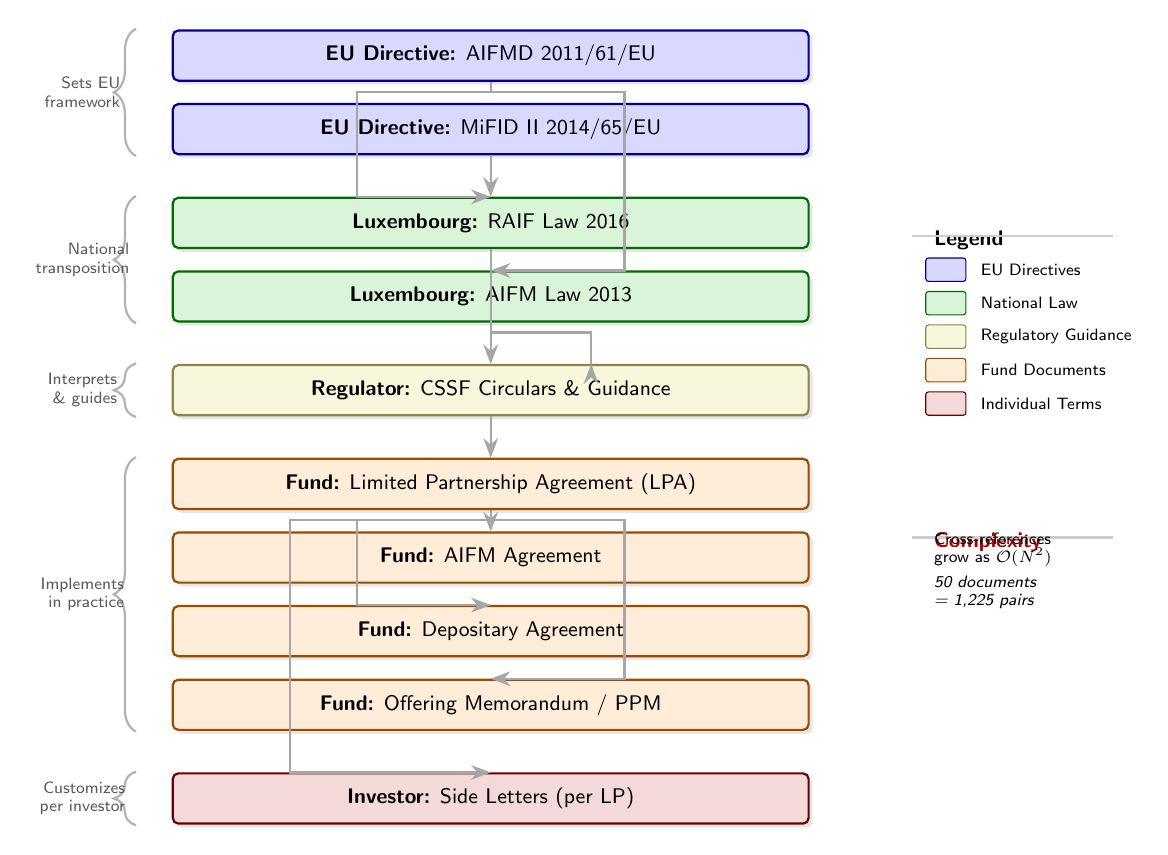
\begin{tikzpicture}[
  scale=0.85,
  transform shape,
  % Layer styles with gradients
  layer/.style={
    rectangle,
    draw=#1!60!black,
    line width=0.8pt,
    minimum width=9.5cm,
    minimum height=0.75cm,
    align=center,
    font=\small\sffamily,
    rounded corners=2pt,
    fill=#1!15,
    drop shadow={shadow xshift=0.5mm, shadow yshift=-0.5mm, opacity=0.2}
  },
  eu/.style={layer=blue},
  national/.style={layer=green!70!black},
  regulatory/.style={layer=yellow!80!black},
  contractual/.style={layer=orange},
  individual/.style={layer=red!70!black},
  % Arrow style
  arrow/.style={
    ->,
    >={Stealth[length=2.5mm]},
    thick,
    draw=gray!70
  },
  % Brace annotation style
  annot/.style={
    font=\scriptsize\sffamily,
    align=right,
    text=gray!70!black
  }
]

% === NODES ===
\node[eu] (aifmd) at (0,0) {\textbf{EU Directive:} AIFMD 2011/61/EU};
\node[eu] (mifid) at (0,-1.1) {\textbf{EU Directive:} MiFID II 2014/65/EU};

\node[national] (raif) at (0,-2.5) {\textbf{Luxembourg:} RAIF Law 2016};
\node[national] (aifm) at (0,-3.6) {\textbf{Luxembourg:} AIFM Law 2013};

\node[regulatory] (cssf) at (0,-5.0) {\textbf{Regulator:} CSSF Circulars \& Guidance};

\node[contractual] (lpa) at (0,-6.4) {\textbf{Fund:} Limited Partnership Agreement (LPA)};
\node[contractual] (aifmag) at (0,-7.5) {\textbf{Fund:} AIFM Agreement};
\node[contractual] (dep) at (0,-8.6) {\textbf{Fund:} Depositary Agreement};
\node[contractual] (om) at (0,-9.7) {\textbf{Fund:} Offering Memorandum / PPM};

\node[individual] (side) at (0,-11.1) {\textbf{Investor:} Side Letters (per LP)};

% === ARROWS ===
\draw[arrow] (aifmd.south) -- ++(0,-0.15) -| ([xshift=-2cm]raif.north) -- (raif.north);
\draw[arrow] (aifmd.south) -- ++(0,-0.15) -| ([xshift=2cm]aifm.north) -- (aifm.north);
\draw[arrow] (mifid.south) -- (raif.north);
\draw[arrow] (raif.south) -- (cssf.north);
\draw[arrow] (aifm.south) -- ++(0,-0.15) -| ([xshift=1.5cm]cssf.north) -- ([xshift=1.5cm]cssf.north);
\draw[arrow] (cssf.south) -- (lpa.north);
\draw[arrow] (lpa.south) -- (aifmag.north);
\draw[arrow] (lpa.south) -- ++(0,-0.15) -| ([xshift=-2cm]dep.north) -- (dep.north);
\draw[arrow] (lpa.south) -- ++(0,-0.15) -| ([xshift=2cm]om.north) -- (om.north);
\draw[arrow] (lpa.south) -- ++(0,-0.15) -| ([xshift=-3cm]side.north) -- (side.north);

% === LEGEND ===
\begin{scope}[shift={(6.5,-3)}]
  \node[font=\small\sffamily\bfseries, anchor=north west] at (0,0.5) {Legend};
  \draw[thick, gray!40] (-0.2,0.3) -- (2.8,0.3);

  \node[rectangle, fill=blue!15, draw=blue!60!black, minimum width=0.6cm, minimum height=0.35cm, rounded corners=1pt] at (0.3,-0.2) {};
  \node[font=\scriptsize\sffamily, anchor=west] at (0.7,-0.2) {EU Directives};

  \node[rectangle, fill=green!70!black!15, draw=green!70!black!60!black, minimum width=0.6cm, minimum height=0.35cm, rounded corners=1pt] at (0.3,-0.7) {};
  \node[font=\scriptsize\sffamily, anchor=west] at (0.7,-0.7) {National Law};

  \node[rectangle, fill=yellow!80!black!15, draw=yellow!80!black!60!black, minimum width=0.6cm, minimum height=0.35cm, rounded corners=1pt] at (0.3,-1.2) {};
  \node[font=\scriptsize\sffamily, anchor=west] at (0.7,-1.2) {Regulatory Guidance};

  \node[rectangle, fill=orange!15, draw=orange!60!black, minimum width=0.6cm, minimum height=0.35cm, rounded corners=1pt] at (0.3,-1.7) {};
  \node[font=\scriptsize\sffamily, anchor=west] at (0.7,-1.7) {Fund Documents};

  \node[rectangle, fill=red!70!black!15, draw=red!70!black!60!black, minimum width=0.6cm, minimum height=0.35cm, rounded corners=1pt] at (0.3,-2.2) {};
  \node[font=\scriptsize\sffamily, anchor=west] at (0.7,-2.2) {Individual Terms};
\end{scope}

% === ANNOTATIONS (LEFT SIDE) ===
\draw[decorate, decoration={brace, amplitude=8pt, mirror}, thick, gray!60]
  (-5.3,0.4) -- (-5.3,-1.5)
  node[midway, annot, xshift=-0.8cm] {Sets EU\\framework};

\draw[decorate, decoration={brace, amplitude=8pt, mirror}, thick, gray!60]
  (-5.3,-2.1) -- (-5.3,-4.0)
  node[midway, annot, xshift=-0.8cm] {National\\transposition};

\draw[decorate, decoration={brace, amplitude=8pt, mirror}, thick, gray!60]
  (-5.3,-4.6) -- (-5.3,-5.4)
  node[midway, annot, xshift=-0.8cm] {Interprets\\\& guides};

\draw[decorate, decoration={brace, amplitude=8pt, mirror}, thick, gray!60]
  (-5.3,-6.0) -- (-5.3,-10.1)
  node[midway, annot, xshift=-0.8cm] {Implements\\in practice};

\draw[decorate, decoration={brace, amplitude=8pt, mirror}, thick, gray!60]
  (-5.3,-10.7) -- (-5.3,-11.5)
  node[midway, annot, xshift=-0.8cm] {Customizes\\per investor};

% === COMPLEXITY ANNOTATION (RIGHT SIDE) ===
\begin{scope}[shift={(6.5,-7.5)}]
  \node[font=\small\sffamily\bfseries, anchor=north west, text=red!70!black] at (0,0.5) {Complexity};
  \draw[thick, gray!40] (-0.2,0.3) -- (2.8,0.3);

  \node[font=\scriptsize\sffamily, anchor=west, text width=2.5cm, align=left] at (0,-0.2) {
    Cross-references\\
    grow as $\mathcal{O}(N^2)$\\[0.3em]
    \textit{50 documents}\\
    \textit{= 1,225 pairs}
  };
\end{scope}

\end{tikzpicture}
\caption{Regulatory and contractual hierarchy in Luxembourg fund structures. EU directives establish the framework; national law transposes requirements; regulatory guidance interprets them; fund documents implement specific terms; and side letters customize arrangements per investor. Each layer may create exceptions to layers above, within permitted limits. The cross-reference complexity between $N$ documents grows quadratically, creating verification challenges that formal methods can address.}
\label{fig:hierarchy}
\end{figure*}


\end{document}
